\chapter{实验评估}

    本章将展示上一章阐述方法的实验结果。对总体性能进行评估,对关键步骤进行考察,对典型图像进行展示。我们将分为视觉(~\ref{sec:visualize}节)和定量(~\ref{sec:analyze}节)两种方式分别评价异常定位和分类的性能,然后,我们将深入模型,解释讨论在学习过程中,模型学习到的信息(\ref{sec:lookInto}节)。在此之前,本章将先说明实验的数据集和实验环境。

\section{数据和环境说明}
    \label{sec:data}
    \subsection{数据集说明} % (fold)
    本实验共包含两个数据集。第一个是杜克大学\cite{srinivasan2014fully}收集的公开数据集。它包含45名去身份化的被试,15名正常被试,15名患有AMD的被试,以及15名有DME病症的被试。对每一名被试的视网膜中心区进行扫描成像,再从扫描像中挑选若干张较有区分度的图像加入杜克数据集中。第二个数据集是北京医院数据集,本实验室与北京医院合作,获取一批临床数据。该批数据的每张图片,都采集于不同患者的视网膜。

    两个数据集相比,杜克数据集的数据较为干净,后者对数据预处理的要求更高。北京医院数据集来源于各不相同的患者,所以多样性更大。且该数据集与实际应用场景较为接近,但规模较小。两个数据集中,每一类的具体数量分布见表.
    \begin{table}[htb]
        \centering
        \caption[数据集说明]{杜克大学数据集合北京医院数据集在健康NOR,老年黄斑变性AMD,黄斑水肿DME三类上的分布}
        \label{tab:dataset}
        \begin{tabularx}{.75\linewidth}{lXXXX}
            \toprule[1.5pt]
            {\heiti 文件名} & {\heiti NOR} & {\heiti AMD} & {\heiti DME} & 共计\\\midrule[1pt]
            杜克大学数据集 & 1407 &723 & 1101 & 3231\\
            北京医院数据集 & 213  &168 & 297  & 678\\
            \bottomrule[1.5pt]
        \end{tabularx}
    \end{table}



    % \subsection{数据预处理}
    % \subsection{数据后处理}
    \subsection{实验环境}
    本实验使用MATLAB语言,在MATLAB2014b上运行通过。其中,0范数下的优化问题使用了~\inlinecite{lee2007efficient}提出的快速算法。针对本应用场景的主要问题是内存空间不足,笔者对程序的空间使用进行了优化,比如主成分分析算法使用了上一章接介绍的改进算法来适应高维矩阵,或调整矩阵乘法降低计算复杂度等。本实验的算法瓶颈在标签一致的字典学习过程。目前本算法不支持多线程运行。

% subsection subsection_name (end)

% \section{环境}
%     \label{sec:environment}
%     \subsection{评价指标}

\section{视觉评估}
    \label{sec:visualize}
    \subsection{选取评估标准}
    本项工作的创新点之一在于,在只有类标签的训练数据上,输出密集图像(dense output),产生位置信息。对于位置信息的评估主要有以下三类方法:方法1.找到图像中心点,输出位置信息,用一组$(x, y)$表示。计算真实位置与输出位置的距离评价。在OCT视网膜图像中,发生病变的区域不一定是一个区域,且中心点难以评判。故没有采用此类方法。 方法2.输出边界框(bounding box),计算真实边界框与输出边界框的重叠比例。该评价指标的问题在于,病变位置的区域难找到客观的确定边界。以上两种评估方法还面临相同的问题:由于推断病变位置需要较强的专家知识,所以两个实验数据集都没有真实的位置信息标注,只能通过视觉评大致观察图像。方法3. 输出热度图(heatmap),该评价指标可以较好的应用于本任务。不仅如此,实际应用中,医生也需要了解逐像素的输出结果。这符合应用场景。我们用像素的灰度表示可能的病变置信度,灰度越大,置信度越高;像素的位置即对应途中推测的病变位置。


    在正文由于篇幅所限,我们每一类只选取2-3个典型代表进行讨论分析。 更多的例子见附录。
    在此,本文用文字描述对视网膜黄斑区使用光学相干成像技术B扫描时,在医学上应观察到的图像特征。~\inlinecite{coscas2009optical}介绍了老年黄斑变性在光学相干成像中的视觉特点。健康的视网膜在OCT成像中,可以看到平滑的突起曲线,在中间有光滑的凹陷(医学上被称作黄斑区中心凹)。健康的图像还可以观察到明显的分层结构。由于上皮层(RPE)与眼球壁结合紧密,通常会在视网膜边界后方形成较暗区域,在上皮层下的血管层,光反射较强,会出现一个亮层。健康图像,在两层分界处平滑清晰,无褶皱。但老年黄斑变性(AMD)的视网膜OCT成像,会发现,交界处的图层褶皱,交界不明显。 糖尿病性黄斑水肿(DME)的图像则显现出视网膜层肿胀(swelling), 囊性黄斑区水肿(cystoid macular edema),和视网膜下积液(subretinal fluid)的症状~\cite{bhagat2009diabetic}具体到图像,则发现典型的糖尿病性黄斑水肿的光学相干成像图像则表现出,在上皮层和血管曾之间出现黑色空洞、中心凹完全消失等表征。


    本文算法流程中,特征提取可以分为两步,主成分分析和标签一致的字典学习与稀疏编码。本节实验将从视觉上评估,1. 特征提取时,虽然维数降低,但是信息几乎没有损失。2. 可逆性,通过特征向量可以重构原图像。重构图像的定量分析,以及特征的判别性将在下一节展示(~\ref{sec:analyze}节)

    \subsection{主成分分析提取特征向量重构图像}

    \subsection{标签一致的字典学习提取特征向量重构主成分}
    在上一小节,实验结果展示了可以通过主成分分析降低维数且几乎不减少信息量,可以重构图像。下面,我们要展示,在标签一致的字典学习一步中,虽然稀疏限制因子$T=10$,即,只用字典中10个原子表达主成分特征,但是,仍然很好的重建了主成分。

    \subsection{特征提取特征重构图像}
    本节最后展示应用算法全部流程后的结果,包括两个部分。1. 特征提取使用特征向量提取图像可以较好的重构原图像;2. 特征向量的判别性,即,只使用$D_{normal}$推测健康特征向量和健康图像,以及展示在源空间中像素相减得到的残差图像,发现实验结果较好的定位了病变位置。

    实验结果展示在图~\ref{fig:recon-all}。第一行是原图像。第二行是由全部字典$D$重建的图像,发现在三类中,都较好的重建了原图的特征,而特征向量非零位只有10位,因此,可以看到,该特征表示保留了原像素空间中较多的信息,是较好的特征提取方法。第三行是由$D_{normal}$拟合健康特征向量,然后投影到原像素空间中的图像,第四行残差图像是第一行与第三行的差。可以看到,对于健康NOR类,几乎残差图像上没有可见灰度,重建的健康图像与本身距离接近;对于老年黄斑变性AMD类,看到第三行拟合了健康图像中的光滑分界层,重建健康图像分界层无褶皱,残差图像在褶皱层位置的灰度清晰可见。对于糖尿病性黄斑水肿DME类,拟合的健康图像中间无空洞,或空洞较少,另外,与AMD不同,DME致使的视网膜形变较大,所以原图中很难找到健康结构,是一类难度更大的样本,但仍然可以看到,在拟合的健康图像中,算法尝试拟合黄斑区中心凹的结构特征,如图~\ref{fig:dme1}。

    \begin{figure}[h]
      \centering%
      \subcaptionbox{NOR典型图像1\label{fig:norm1}}[0.5 \textwidth] %标题的长度,超过则会换行,如下一个小图。
        {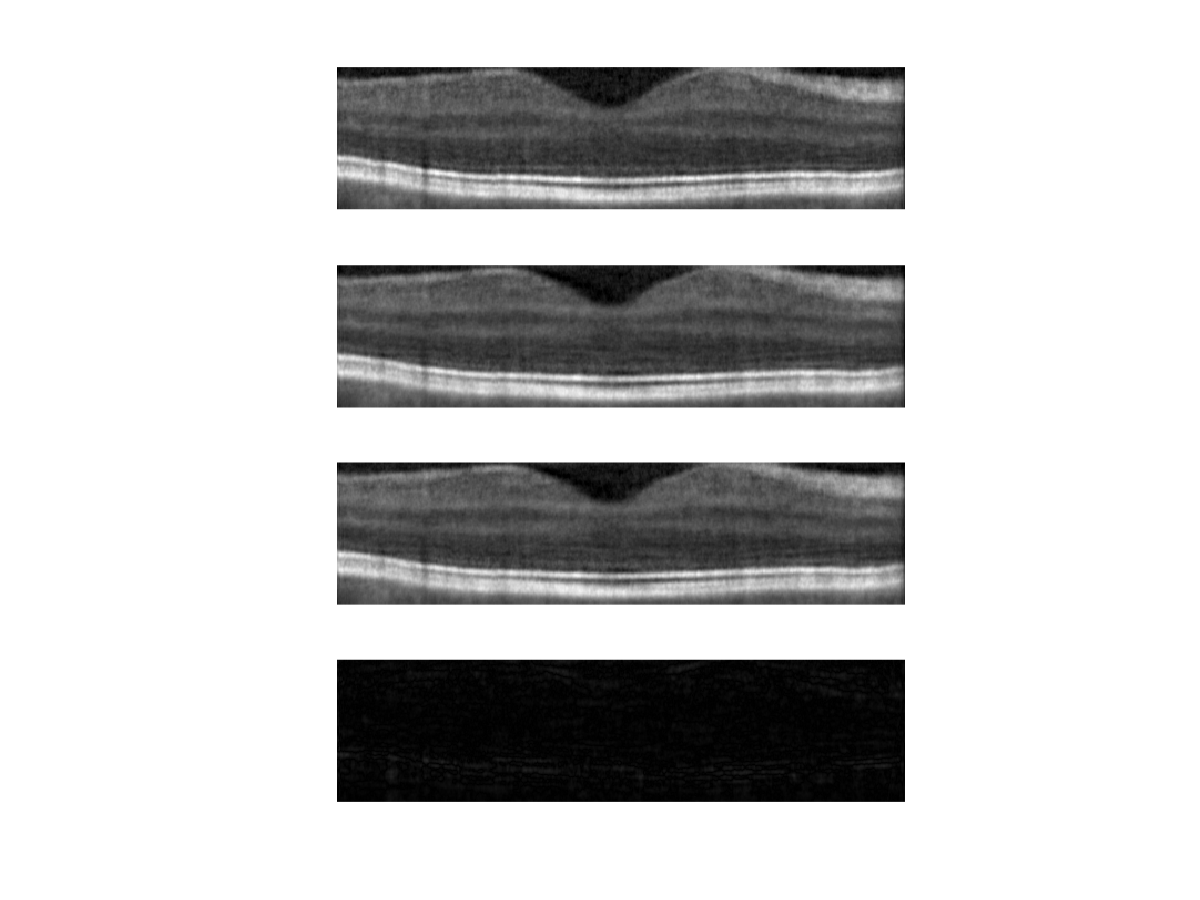
\includegraphics[width=0.5 \textwidth]{nor1}} %
      \hspace{-4em}%
      \subcaptionbox{NOR典型图像2\label{fig:norm2}}[0.5 \textwidth] %标题的长度,超过则会换行,如下一个小图。
        {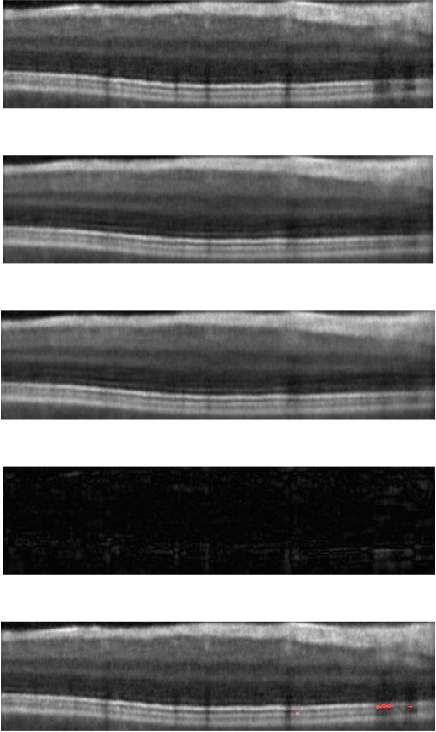
\includegraphics[width=0.5 \textwidth]{nor2}} \\
      \vspace{1em}
      \subcaptionbox{AMD典型图像\label{fig:amd1}}[0.5 \textwidth] %标题的长度,超过则会换行,如下一个小图。
        {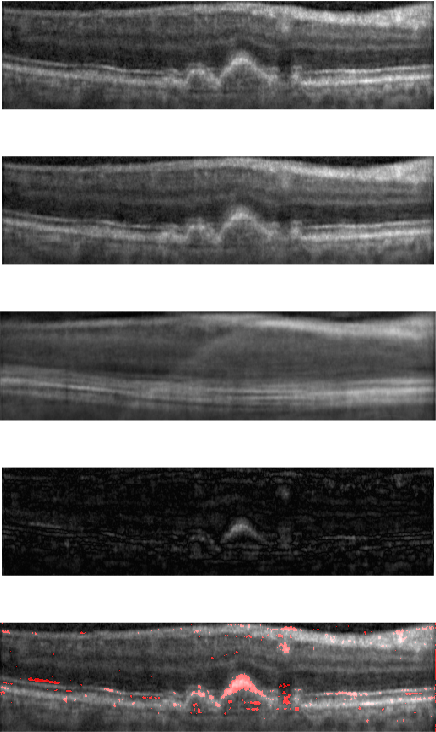
\includegraphics[width=0.5 \textwidth]{amd1}} %
      \hspace{-4em}%
      \subcaptionbox{AMD典型图像\label{fig:amd2}}[0.5 \textwidth] %标题的长度,超过则会换行,如下一个小图。
        {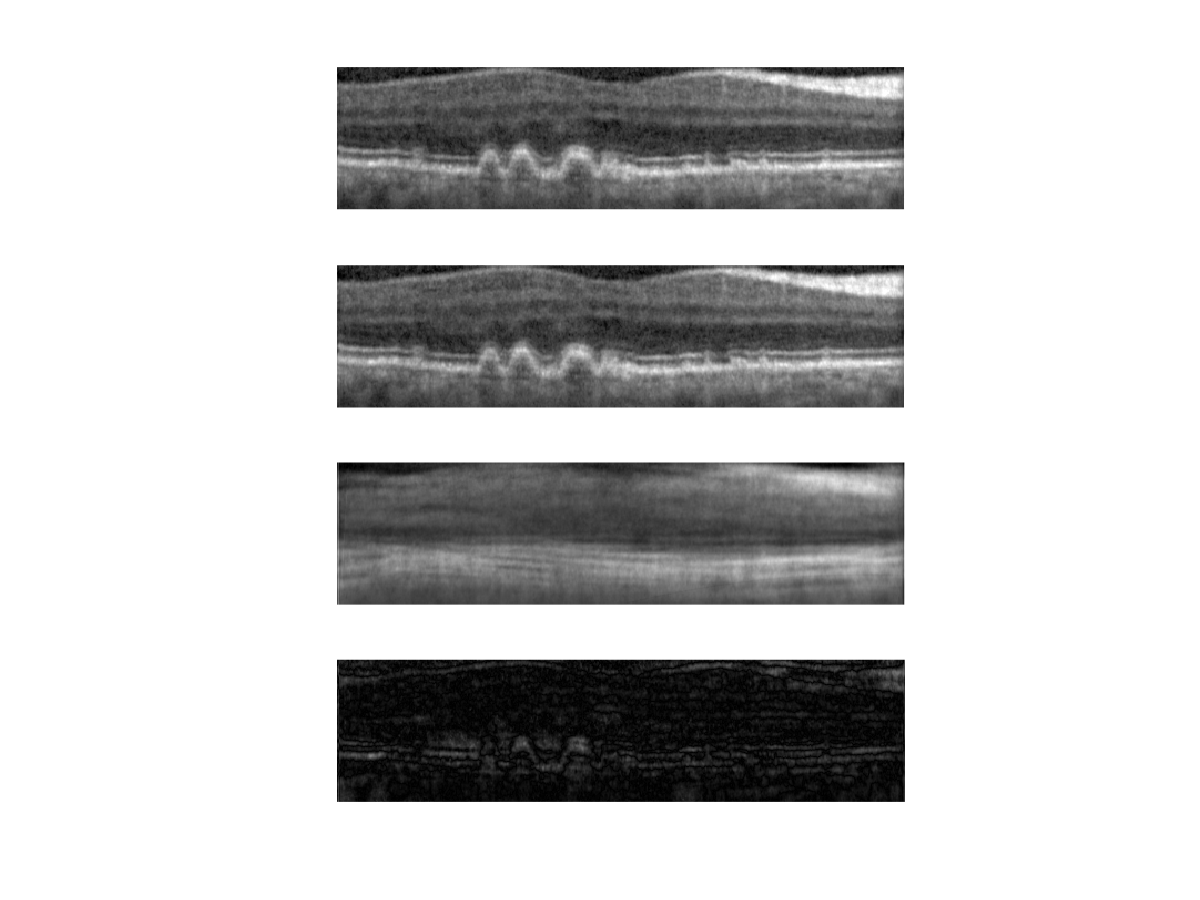
\includegraphics[width=0.5 \textwidth]{amd2}} \\
      \vspace{1em}
      \subcaptionbox{DME典型图像1\label{fig:dme1}}[0.5 \textwidth] %标题的长度,超过则会换行,如下一个小图。
        {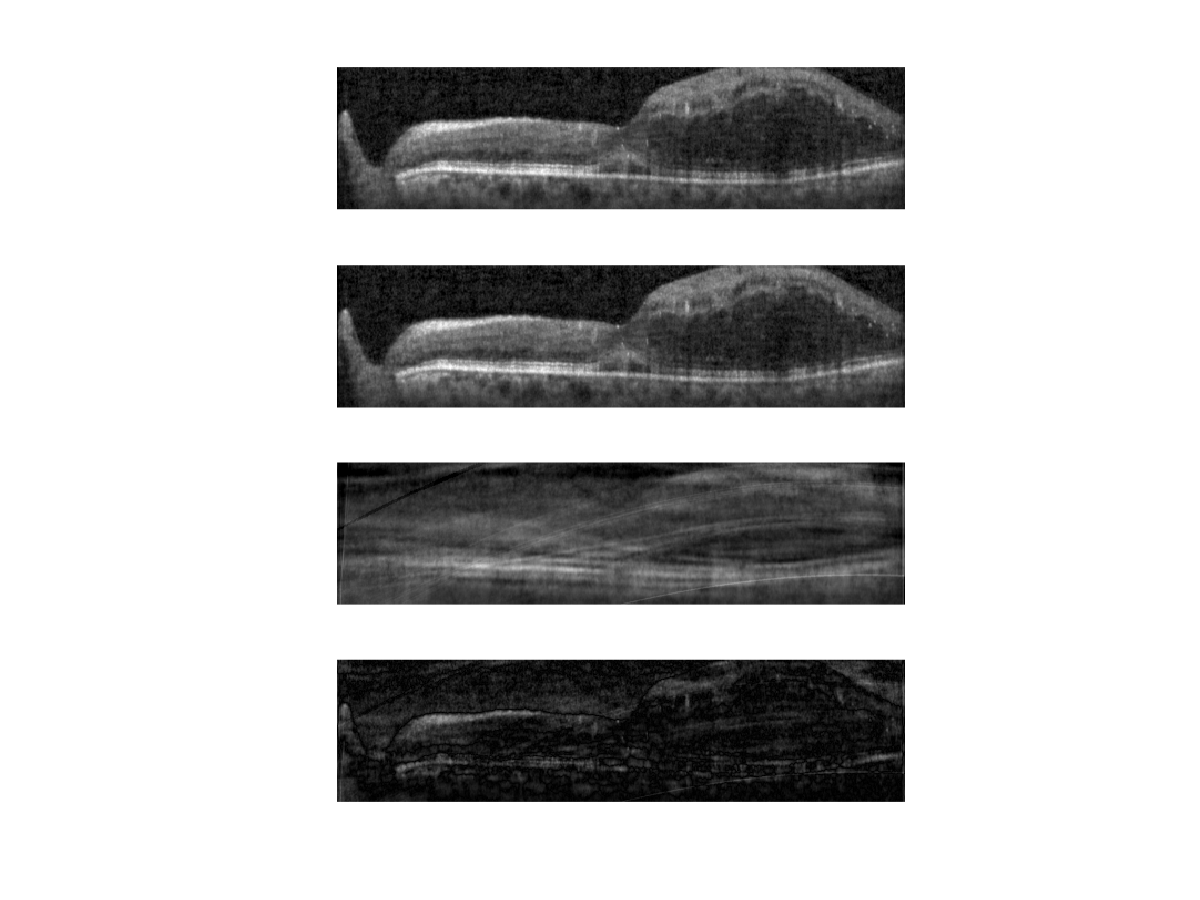
\includegraphics[width=0.5 \textwidth]{dme1}} %
      \hspace{-4em}%
      \subcaptionbox{DME典型图像2\label{fig:dme2}}[0.5 \textwidth] %标题的长度,超过则会换行,如下一个小图。
        {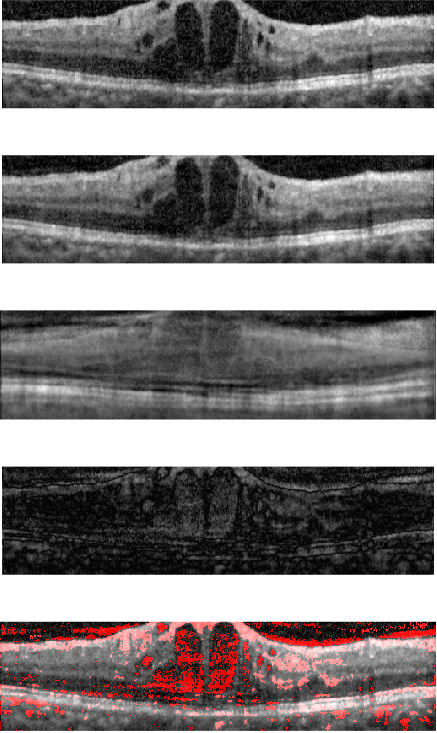
\includegraphics[width=0.5 \textwidth]{dme2}} \\
      \caption[算法完整流程结果]{利用本算法提取特征向量并重建原图像和健康图像。第一行是原图,第二行是重建图像,第三行重建健康图像,第四行是推测病变位置,即第一行和第三行的差。}
      \label{fig:recon-all}
    \end{figure}



    % \subsection{异常定位}
    % \subsection{}

\section{定量评估}
    \label{sec:analyze}
    \subsection{分类}
    汇报在两个数据集上的分类准确率。北京医院数据集是一个较小的数据集,本实验中使用了 两种训练集测试集的划分。在第一种划分中,取2/3数据做训练集,剩余做测试集,同样进行交叉验证。第二种划分,测试集每类随机选取30个,其余做训练集,进行交叉检验。得到各类识别准确率表~\ref{tab:clf-beijing}.表中,mAP表示平均准确率(mean Accuracy Performance),分别将提取的特征向量使用1.标签一致的字典学习中习得的线性分类器 2.支持向量机 两种分类器进行分类。“(2/3+1/3)”表示第一种数据集划分,“(x+30)”表示第二种数据集划分。
    \begin{table}[htb]  
        \centering
        \caption{北京医院数据集}
        \label{tab:clf-beijing}
        \begin{tabularx}{.75\linewidth}{lXXXX}
            \toprule[1.5pt]
            {\heiti 方法} &{\heiti mAP} & {\heiti NOR} & {\heiti AMD} & {\heiti DME}\\\midrule[1pt]
            线性(2/3+1/3) & 0.736  &0.866  &0.515  &0.773 \\
            svm(2/3+1/3) &0.745   &0.866  &0.541  &0.826 \\\midrule[1pt]
            线性(x+30) &0.866   &0.933  &0.733  &0.933 \\
            svm(x+30) &0.888  &0.900 &0.766  &1.000 \\
            \bottomrule[1.5pt]
        \end{tabularx}
    \end{table}
    在本组实验中,当训练样本增加时,无论是线性分类器还是支持向量机的分类性能都有较明显提升。因此推断,在北京医院的数据集上,对于本方法,数据量过小,模型过拟合较严重。当本方法在杜克大学的较大数据集上实验室看到,分类性能进一步提升,印证了推断。

    
    % 比较,讲所有参数
    本实验通过定量分析的方法选取了实验参数。下面对重要参数的选取进行说明和分析。

    \textbf{选取主成分分析维数}. 主成分分析的目的除了去相关性,更主要的功能是降维。这是因为在之后的流程中,标签一致的字典学习是本算法的计算量瓶颈,而它不能处理过高的维数。但是,维数降低的越多,则会使得在主成分分析丢失的信息越多。

    用$\lambda_i$表示从大到小排列的特征值,定义$S_k$表示累计特征值:

    \begin{equation}
    S_k = \frac{\sum_{i = 1}^k |\lambda_i|} {\sum_{i} |\lambda_i|}
    \end{equation}
    得到$S_k $如下表
    \begin{table}[htb]
        \centering
        \caption{PCA维数选取}
        \label{tab:pca-dim}
        \begin{tabularx}{.75\textwidth}{lXXXX}
            \toprule[1.5pt]
            {\heiti $S_k$} &  0.80 & 0.85 & 0.90 &0.95 \\\midrule[1pt]
            {\heiti $k$} & 98 &161 & 345 & 811\\
            \bottomrule[1.5pt]
        \end{tabularx}
    \end{table}
    本试验中选取$S_k = 0.95$时的$k$,即把原来$512*128 = 65536$维的图像降至811维,既大大降低了字典学习的计算量,又选取了尽量多的特征值,并且由$S_k$表明,这811维向量所对应的特征值,贡献了数据集中95\%的变化,是一种折中的参数选取。值得一提的是,本节在这里只提出了一种寻找参数的方法,由于随数据集大小,$S_k$不断变化,$k$的选取会因此不同,但主要考量方面是如上讨论的计算开销与保留的信息量两个角度。

    \textbf{字典大小的选取}。目前对与稀疏编码字典大小的选取没有明确的理论方法。但字典大小影响了分类性能,因此字典大小在训练中应该被作为首要的超越参数(hyper parameter)谨慎选取。
    \begin{table}[htb]
        \centering
        \caption{}
        \label{tab:pca-dim}
        \begin{tabularx}{.75\textwidth}{l|X}
            \toprule[1.5pt]
            PCA=120, 字典大小=150 & 0.911\\
            PCA=120, 字典大小=1500 & 0.921\\\midrule[1pt]
            PCA=811, 字典大小=1200 &0.929\\
            PCA=811, 字典大小=1500 &\textbf{0.946}\\
            \bottomrule[1.5pt]
        \end{tabularx}
    \end{table}
    而经过实验发现,在标签一致的字典 学习算法中,其余参数,如稀疏限制,稀疏系数权重,分类稀疏权重等,对于分类结果都不如字典大小对于分类结果的影响大。经过详尽的参数选取,对于杜克数据集,字典大小取1500时,分类效果最佳。为94.6\%.请注意这只是通过线性分类器得到的分类结果。


    \subsection{重建图像误差}
    本小节从定量的角度分析本算法特征向量的表达性和可逆性。采用的评价指标是在整个数据集上重构图像$X'$与$X$的平均像素差。对主成分分析和稀疏编码两个阶段分别考察,在做完主成分分析之后,直接使用重构算法;以及,计算得到稀疏编码和字典后,利用完整字典重构原图像(表~\ref{tab:recon}中第一行和第三行),重构误差较小。除此之外,还计算了健康拟合之后的平均重构误差。因为我们希望分别比较两个阶段的特征提取,排除彼此影响,因此在表中,二行和第三行的重构误差,并没有与原图做差,而是用全部特征向量$Y$重构得到的$\tilde{Y}$减去健康子空间中拟合得到的特征$Y^{normal}$重构所得$\tilde{Y^{normal}}$的结果。
    \begin{table}[htb]  
        \centering
        \caption{重建图像平均误差}
        \label{tab:recon}
        \begin{tabularx}{.75\linewidth}{lXXX}
            \toprule[1.5pt]
            {\heiti 文件名} & {\heiti NOR} & {\heiti AMD} & {\heiti DME}\\\midrule[1pt]
            主成分分析(all) &7.54 &7.41 &7.41\\
            稀疏编码(all) & 5.24 &6.20 &6.51\\
            稀疏编码(NOR) & 5.81  &\textbf{18.2} & \textbf{20.5} \\
            \bottomrule[1.5pt]
        \end{tabularx}
    \end{table}

    从表中可以发现,两个阶段的特征提取相比,主成分分析的重构误差较大,信息在该阶段的损失相较于后者更大。对比第二行和第三行,健康NOR类的重构误差没有太大变化,说明用健康类的子字典就可以表达健康特征向量子空间;老年黄斑变性AMD和糖尿病性黄斑水肿DME的病态图像,进行健康特征向量拟合并投影回像素空间后,重构误差明显增大,(增幅约290\% - 315\%),这说明,健康的特征向量原子所构成的健康子空间,不能表达出某些病态部分,而这部分却可以被原来带有该类别标签的字典原子表示。根据以上分析,可以认为,本实验说明了提取的特征有一定的判别性,但也保存了图像的信息。

\section{理解模型}
    \label{sec:lookInto}
    在前面的章节,我们从定量和定性两个角度证明了本工作中算法的有效性,并证明了算法动机中对特征向量提出的特性:去相关性、判别性、可逆性。与此同时,我们还希望理解,在学习过程中,不同的构件分别学到了何种知识。这是一个难以回答的问题,本节用可视化的方法,试图剖析这个问题,深入模型内部,理解学习过程。同时,在窥探模型的过程中,进一步印证特征向量符合三条特性。在~\ref{sec:param}小节中,列出了主要参数的选取和理由。

    \subsection{PCA降维}
    % PCA的Coeff图
    主成分分析求得的特征向量方向,是数据集上数据分布变化最大的方向,且相互正交。可视化最大的10个特征值所对应的特征向量如图~\ref{fig:pca-coeff}
    \begin{figure}[H] % use float package if you want it here
      \centering
      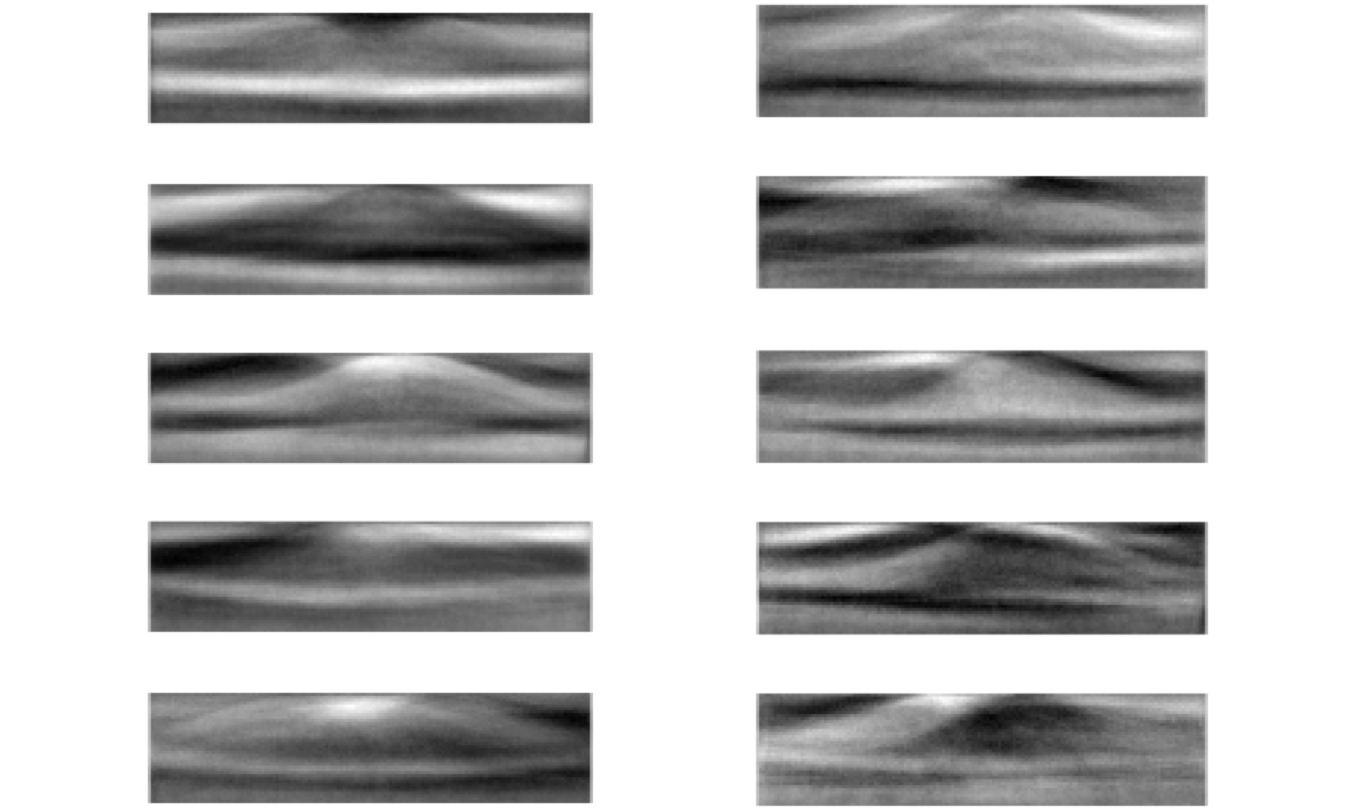
\includegraphics[width=\textwidth]{base}
      \caption[PCA特征向量]{主成分分析最大的10个特征值对应的特征向量}
      \label{fig:pca-coeff}
    \end{figure}
    观察发现特征向量之间的形态差别很大,这是由于主成分分析的特征值互相正交,因此也在这组基下的特征向量的去相关性。

    另一方面,观察在这组特征值下的系数,把该类的所有系数表示在一张茎叶图中,如图~\ref{fig:pca-stem}。有两个观察,首先,在这些方向上的投影分布,如理论,有明显的由大到小的趋势;其次,可以看到,每一类的系数分布略有不同。从一个侧面说明,PCA提取的特征向量也有一定的判别性。

    \begin{figure}[H] % use float package if you want it here
      \centering
      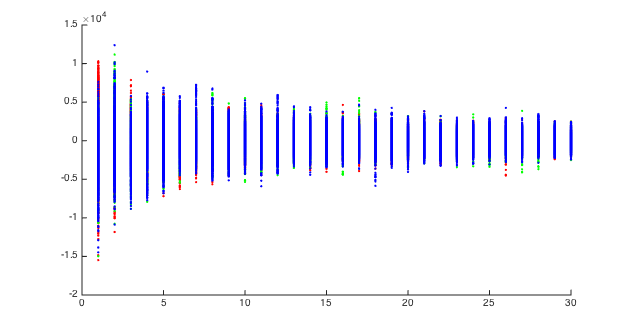
\includegraphics[width=\textwidth]{pca-score}
      \caption[PCA系数分布]{主成分分析最大的30个特征值对应的特征向量上的投影分布。红色代表NOR类,绿色代表AMD类,蓝色代表DME类。}
      \label{fig:pca-stem}
    \end{figure}

    最后,展示主成分分析得到的平均位移图像。这个图像是健康,老年黄斑变性,糖尿病性黄斑水肿三类图像求平均值所得。仍然可以隐约看到完整视网膜成像的结构,平均位移图像形态较为清晰整齐,可以隐约看到视网膜黄斑区中心凹,隐约看到上皮层和血管层间的分界层的亮纹。如上说明,数据预处理,对齐降噪,裁剪等步骤起了较好的效果。
    \begin{figure}[H] % use float package if you want it here
      \centering
      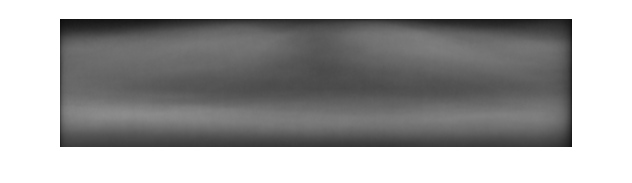
\includegraphics[width=\textwidth]{pca-mean}
      \caption[PCA平均位移图像]{可见黄斑区中心凹,可见大致轮廓,可见不同层交接处的亮纹。}
      \label{fig:pca-mean}
    \end{figure}


    \subsection{字典学习}
    % 字典图
    可视化学习到的字典原子,每一类随机选取了9个原子并重建到像素空间中,如图~\ref{fig:dl-dict}。注意到,虽然训练在学习过程中是一起训练的,所有原子的训练数据是全部类别的训练样本,但是,由于标签一致的限制条件,使得字典的每个原子有标签,因此,每一类字典原子都能看到与其它类别的原子的显著区别。

    \begin{figure}[H]
      \centering%
      \subcaptionbox{NOR\label{fig:dl-nor}}[\textwidth] %标题的长度,超过则会换行,如下一个小图。
        {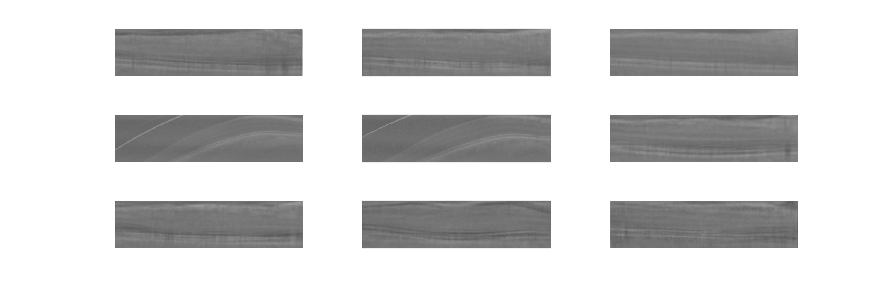
\includegraphics[width=\textwidth]{dict-nor}} \\
        \vspace{1em}
      \subcaptionbox{AMD\label{fig:dl-amd}}[\textwidth] %标题的长度,超过则会换行,如下一个小图。
        {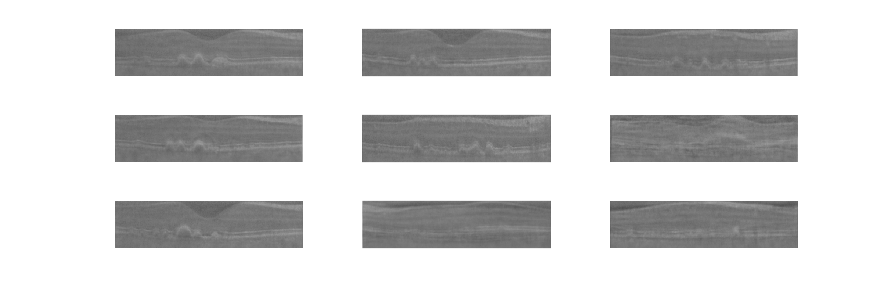
\includegraphics[width=\textwidth]{dict-amd}} \\
        \vspace{1em}
      \subcaptionbox{DME\label{fig:dl-dme}}[\textwidth] %标题的长度,超过则会换行,如下一个小图。
        {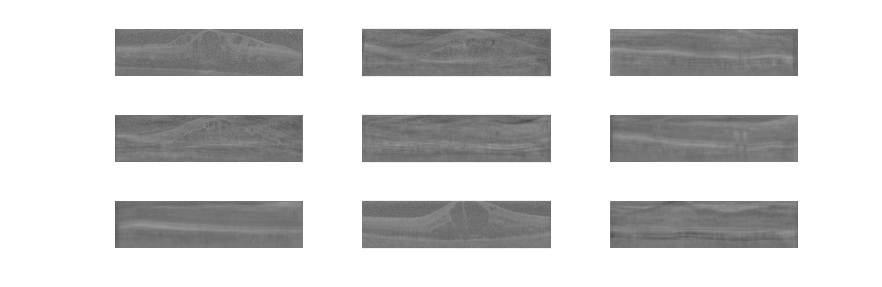
\includegraphics[width=\textwidth]{dict-dme}} \\
      \caption[字典原子可视化]{学习到的字典原子转换到像素空间中。虽然训练是一起的,但是不同的标签使它们学习到了不同类别的特征,不同标签之间的原子有较大区别。}
      \label{fig:dl-dict}
    \end{figure}

    观察稀疏编码系数的直观表示,把每类图像的每一个样本提取的稀疏系数画在同一个坐标轴上,可以观察到,不同类别的稀疏系数有明显区别,真实类别倾向于使用具有该类别标签的原子表示。对比图~\ref{fig:pca-stem},发现字典学习一步得到的特征表示,不同类之间的区别性大很多。除此,主成分分析中方差则由大至小递减较明显,这一性质不利于分类器分类。在稀疏编码之后,我们发现,每一维上的稀疏分布方差几乎相等,从而克服了如上问题。

    \begin{figure}[H]
      \centering%
      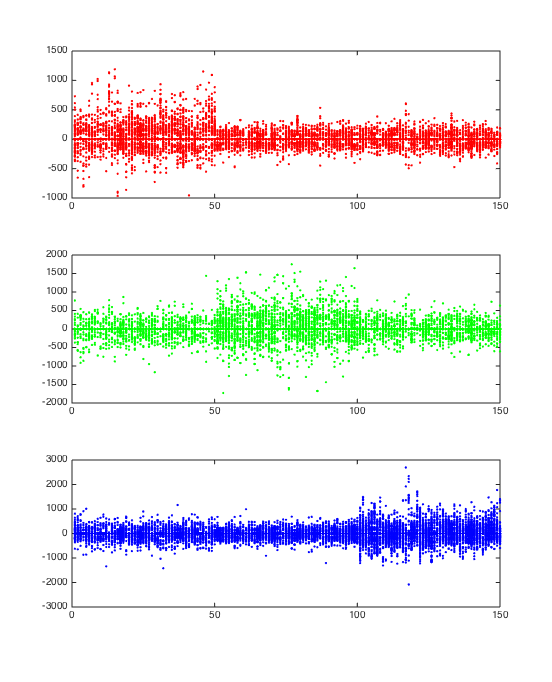
\includegraphics[width = 0.75\textwidth]{dl-allsc}
      \caption[稀疏表示分布]{红色表示NOR,绿色表示AMD,蓝色表示DME。每一类的分布模式差别较大,都倾向于使用真实所属类别的原子编码自己。同时,不同维数的方差相较主成分分析投影结果平均很多,有利于分类。}
      \label{fig:dl-allsc}
    \end{figure}

    \subsection{稀疏性}
    % pca之后的stem图
    研究表明,稀疏性是图像分布的自然属性,可以借助于此提高图像识别等任务的表现。因此,理解模型时希望直观比较特征向量的稀疏程度。

    图~\ref{fig:sc-pca}是对一张随机样本,在进行主成分分析之后,把前180维特征向量方向上的投影长度画在了茎叶图上。发现,虽然通过主成分分析维数降低了,但是并没有特征的稀疏性。
    \begin{figure}[H]
      \centering%
      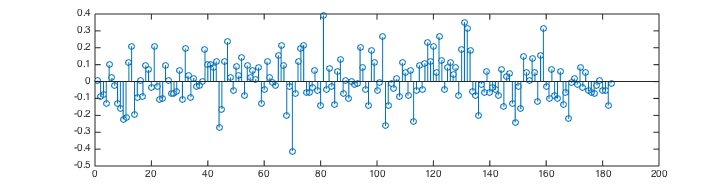
\includegraphics[width = \textwidth]{pca-sc}
      \caption{PCA投影分布}
      \label{fig:sc-pca}
    \end{figure}
    
    标签一致的字典学习与稀疏编码之后,得到的稀疏系数使用同样的方法在茎叶图上表示。仅对每一类其中一个样本的系数茎叶图进行展示,如图~\ref{fig:sc-dict}。蓝色部分是提取特征向量得到的$y_i$,字典里所有原子都参与了优化问题。发现相比于主成分分析后的特征,稀疏编码得到的$y_i$要稀疏很多,且非0部分基本集中在有相同标签的字典原子上。红色部分是利用$D^{normal}$重构的$y^{normal}_i$。这里放松了稀疏限制,但发现,求解所得的表示仍然相较于主成分分析特征~\ref{fig:sc-pca}中的表示更稀疏。且,原来的表示中非0的点,通常在拟合健康特征的时候,该部分特征得到了增强。 

    % 稀疏的stem图
    \begin{figure}[H]
      \centering%
      \subcaptionbox{NOR\label{fig:sc-nor}}[0.3\textwidth] %标题的长度,超过则会换行,如下一个小图。
        {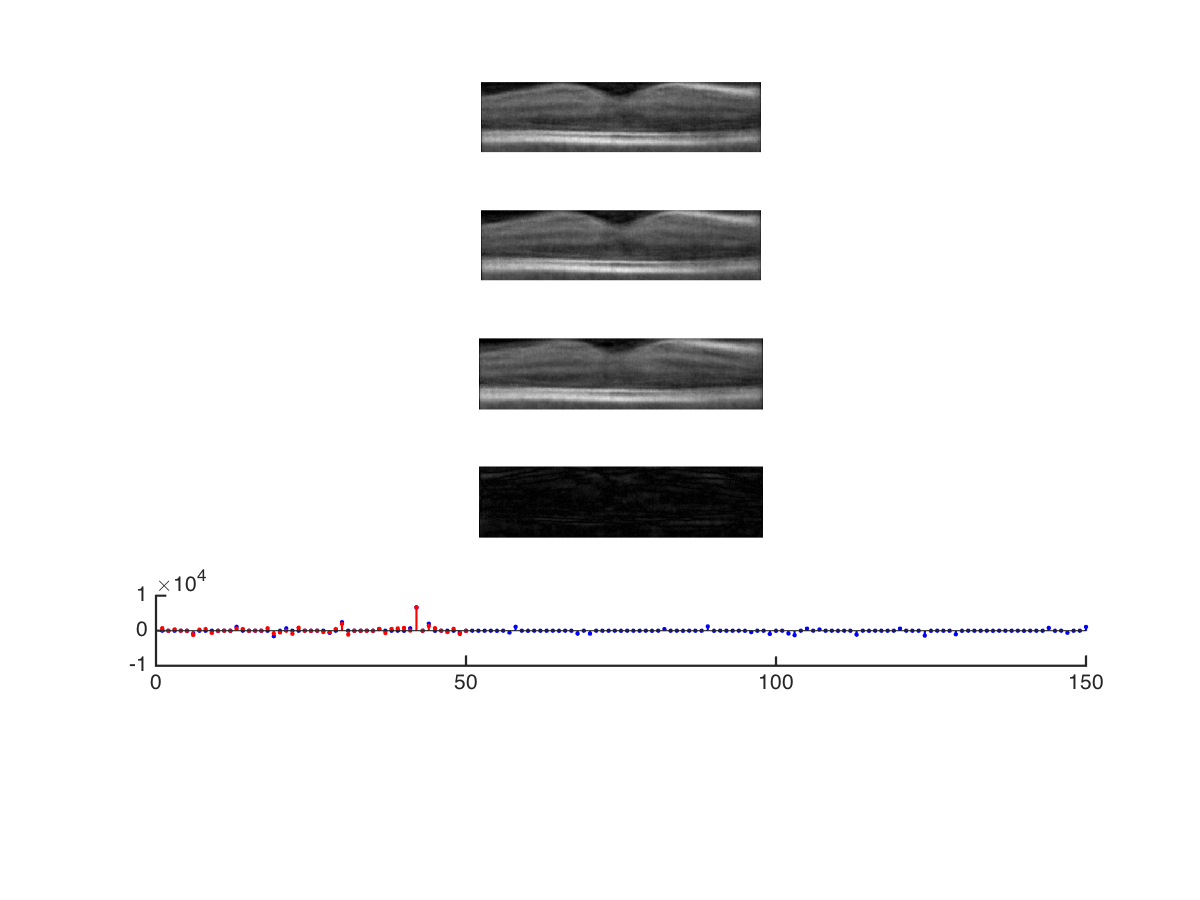
\includegraphics[width=0.3\textwidth]{sc-nor}} 
        % \vspace{1em}
      \subcaptionbox{AMD\label{fig:sc-amd}}[0.3\textwidth] %标题的长度,超过则会换行,如下一个小图。
        {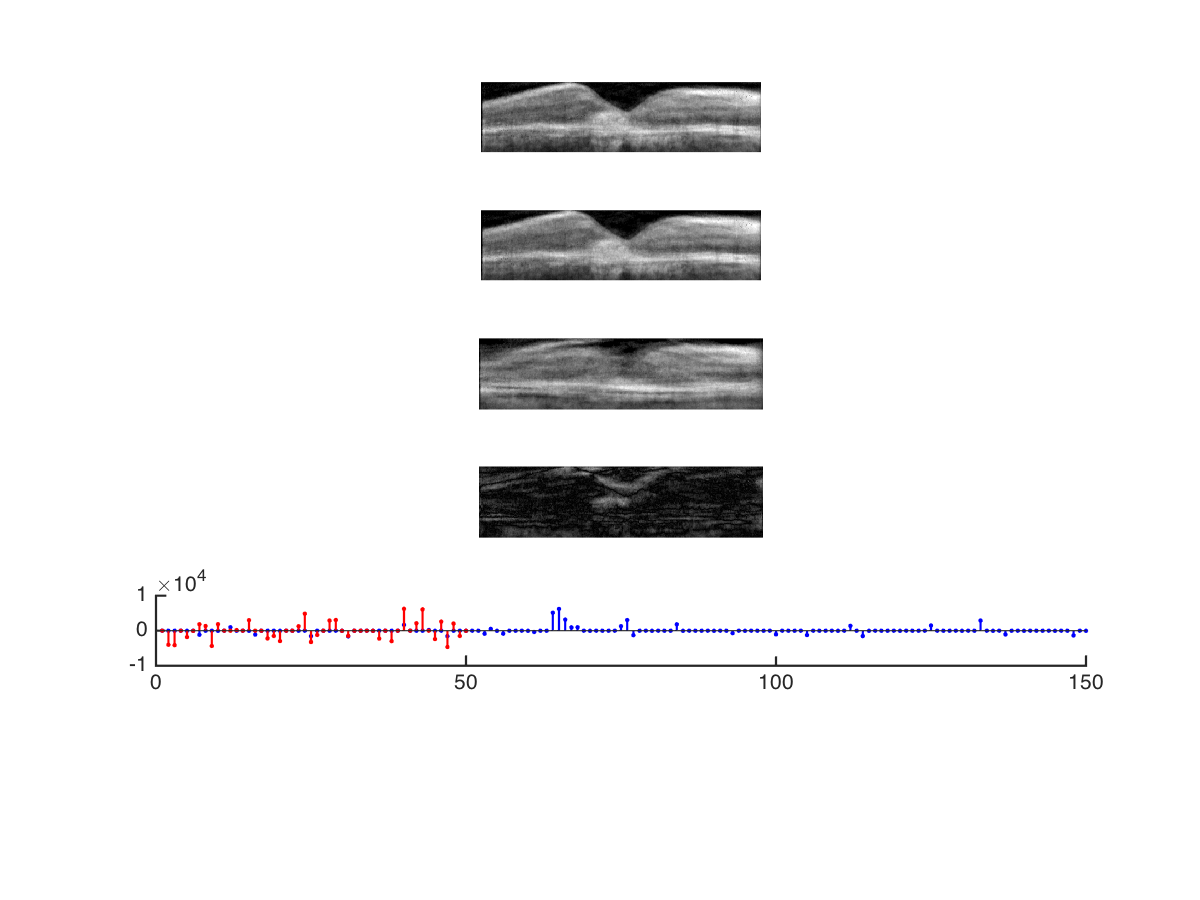
\includegraphics[width=0.3\textwidth]{sc-amd}} 
        % \vspace{1em}
      \subcaptionbox{DME\label{fig:sc-dme}}[0.3\textwidth] %标题的长度,超过则会换行,如下一个小图。
        {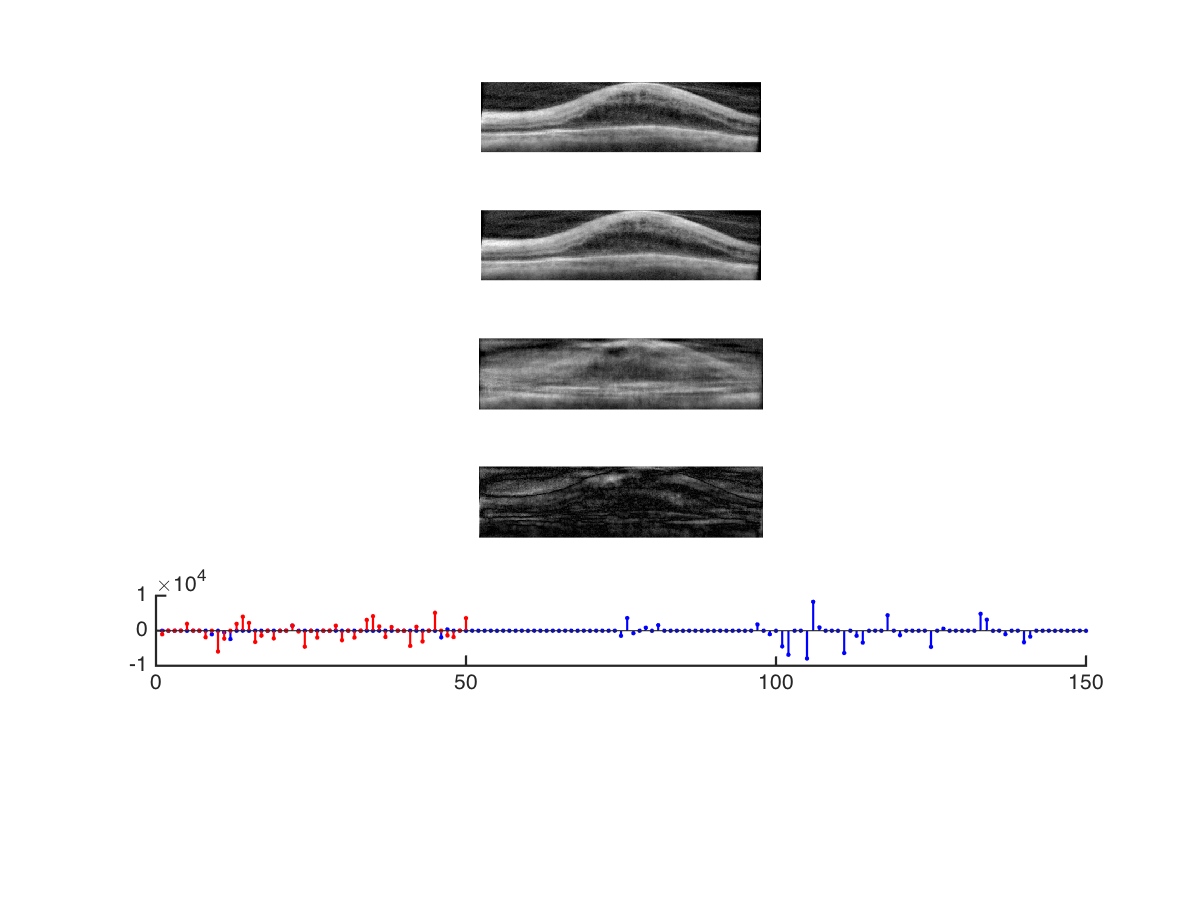
\includegraphics[width=0.3\textwidth]{sc-dme}} 
      \caption[稀疏编码]{蓝色表示使用全部字典的稀疏表示,红色表示仅使用健康标签字典的稀疏表示。}
      \label{fig:sc-dict}
    \end{figure}

\section{本章小结}
    在上一章,本文提出了提取的特征的几个性质,在本章得到了证明。通过视觉评估印证了可逆性,通过定量评估印证了判别性和可逆性,最后,通过理解模型,我们郑光明了特征的稀疏性并试图理解模型学习到的知识。在实验结果展示与比较过程中,也说明了一些重要参数的选取方法。实验证明,本算法得到的实验结果,基本符合理论预期。


% section section_name (end)